
Este capítulo descreve o processo de implementação dos algoritmos de dimensionamento, detalhados nos capítulos anteriores. 
Descreve-se a seguir a arquitetura aplicação desenvolvida, as tecnologias utilizadas e a tradução da lógica de cálculo em código python.

\subsection{Arquitetura e tecnologia}
O desenvolvimento e implementação da aplicação baseia-se numa arquitetura modular, dividida entre o \textit{Backend}, onde se integra a lógica de cálculo e de dados, 
e o \textit{Frontend}, onde se integra a interface de interação entre utilizador e aplicação, ver a estrutura de ficheiros apresentada em Listing 5.

\subsubsection{Arquitetura MVT e Serviços}
A aplicação foi construída sobre a framework web Django \cite{DjangoDocs}, baseada na linguagem Python. 
O Django adota o padrão de desenho de software Modelo-Vista-Template (MVT), que promove o desenvolvimento rápido e um \textit{design} pragmático através da separação de responsabilidades. 
No contexto desta aplicação, o padrão MVT organiza-se da seguinte forma:

%\begin{enumerate}
    \begin{enumerate}
        \item \textbf{Modelo (Model):} É a camada de acesso aos dados. Define a estrutura da base de dados através de classes Python simples, abstraindo a complexidade de transacionar SQL diretamente. Na aplicação desenvolvida, os modelos gerem, por exemplo, o registo do histórico de cálculos do utilizador (\texttt{HistoricoCalculo}) e as configurações visuais do sistema (\texttt{SystemConfiguration}).
        \item \textbf{Vista (View):} É o "cérebro" da resposta web. Recebe o pedido HTTP feito pelo utilizador (por exemplo, a submissão do formulário de dimensionamento de uma viga), orquestra o processamento desses dados (comunicando com os Modelos ou com a camada de Serviços) e, no final, seleciona qual o Template a ser renderizado com os resultados da operação para devolver como resposta.
        \item \textbf{Template:} Corresponde à camada de apresentação ao utilizador (frontend). Consiste em ficheiros HTML dinâmicos que utilizam uma linguagem de \textit{tags} própria (Django Template Language) para colocar as variáveis calculadas geradas pela Vista no sítio certo do interface gráfico.
    \end{enumerate}
%\end{enumerate}

Para fazer face à especificidade de engenharia do presente trabalho, a arquitetura MVT padrão do Django foi complementada por uma camada de \textbf{Serviços} explícita. Esta decisão arquitetural visa encapsular a pesada complexidade matemática dos algoritmos de dimensionamento estrutural, isolando-a da lógica de encaminhamento web das \textit{Views}. Esta abordagem modular garante um código mais testável, escalável e com uma clara separação de responsabilidades, e encontra-se ilustrada na Figura \ref{fig:arquitetura_mvt_cap5}.

\begin{figure}[H]
  \centering
  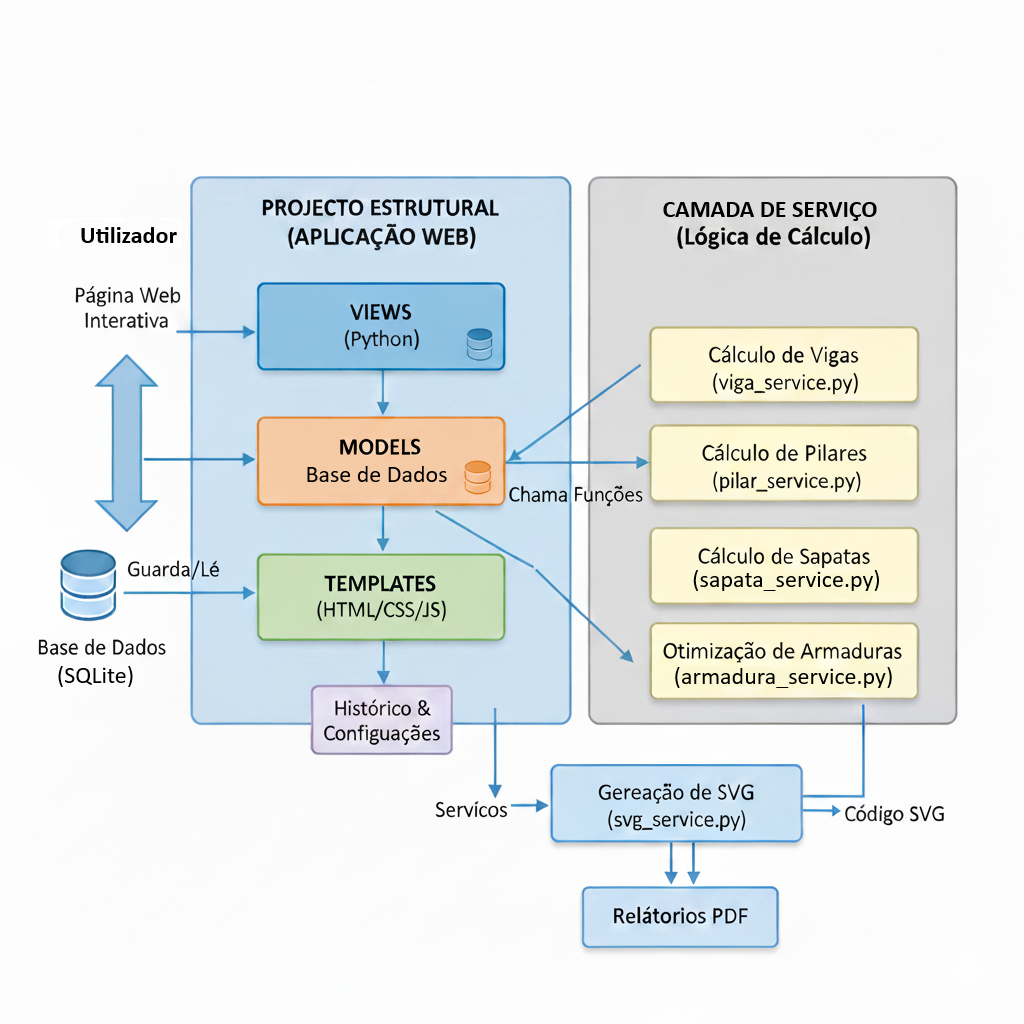
\includegraphics[width=1\textwidth]{Figuras/arquitetura_mvt.png}
  \caption{Diagrama da arquitetura MVT + Serviços da aplicação desenvolvida.}
  \label{fig:arquitetura_mvt_cap5}
\end{figure}

\subsubsection{Tecnologias Backend}
\begin{enumerate}
    \item \textbf{Python 3.10} \cite{PythonDocs}: linguagem base, adequada a cálculos numéricos.
    \item \textbf{Django ORM}: abstrai operações SQL para modelos como \texttt{HistoricoCalculo}.
    \item \textbf{Serviços modulares}: lógica EC2 isolada em \texttt{services/}, facilitando testes unitários.
\end{enumerate}

\subsubsection{Tecnologias Frontend}
\begin{enumerate}
\item \textbf{Templates Django}: HTML dinâmico com injeção de dados dos serviços.
\item \textbf{CSS3}: variáveis personalizáveis para temas claro/escuro.
\item \textbf{SVG}: geração vetorial de desenhos técnicos \cite{DaileySVG}.
\item \textbf{JavaScript}: validação de formulários e interatividade \cite{PortelaAvancado,MDNWeb}.
\end{enumerate}

\newpage
\begin{lstlisting}[basicstyle=\ttfamily\normalsize, moredelim={[is][\color{blue}\bfseries]{@}{@}}, morecomment={[l]\#}, commentstyle=\color{codegreen}\itshape, caption={Estrutura de ficheiros do projeto Django}, label={lst:estrutura_1}]

@TeseFinal/@
|-- manage.py
|-- requirements.txt
|-- @projeto_estrutural/@
|   |-- settings.py
|   |-- urls.py
|   |-- wsgi.py
|   |-- asgi.py
|-- @calculos/@
    |-- models.py                   # Base de Dados
    |-- views.py                    # Controlador HTTP
    |-- urls.py
    |-- forms.py
    |-- tests.py
    |-- @services/@                   # Camada de Servicos
        |-- viga_service.py
        |-- pilar_service.py
        |-- sapata_service.py
        |-- armadura_service.py
    |-- @templates/calculos/@          # Interface
    |   |-- base.html
    |   |-- index.html
    |   |-- viga_dimensionamento.html
    |   |-- pilar_dimensionamento.html
    |   |-- sapata_dimensionamento.html
    |   |-- historico.html
    |   |-- historico_detalhe.html
    |   |-- configuracao.html
    |   |-- relatorio_pdf.html
    |-- @static/calculos/@            # Temas visuais
        |-- style.css
        |-- @icons/@
            |-- artic.svg
            |-- encab.svg
            |-- livre.svg
\end{lstlisting}

\subsection{Implementação dos algoritmos}

A tradução dos modelos teóricos, apresentados no capítulo 4, para código Python são seguidamente apresentados:

\begin{enumerate}
    \item Algoritmo 1 - viga:\\
    O \texttt{viga\_service.py} implementa o dimensionamento completo à flexão simples. O algoritmo inicia-se com a verificação dos limites de ductilidade, momento reduzido $\mu$. A sua principal característica é o ciclo de \textit{refinamento automático}. Após uma estimativa inicial, o sistema identifica o diâmetro da solução ótima e, se este diferir do assumido, recalcula a altura útil $d$, e a área de aço para betão necessária, garantindo total coerência entre o cálculo e a solução construtiva. Por fim, valida a área obtida comparando-a com a armadura mínima regulamentar.

    \item Algoritmo 2 - pilar:\\
    O \texttt{pilar\_service.py} contém a lógica para a análise de estabilidade. Verifica a esbelteza $\lambda$, e, se necessário, aplica o Método da Curvatura Nominal para calcular os efeitos de segunda ordem. A função \texttt{\_dimensionar\_pilar\_rigoroso} utiliza um método numérico iterativo para encontrar a profundidade do eixo neutro e o momento resistente da secção.

    \item Algoritmo 3 - sapata:\\
    O \texttt{sapata\_service.py} reflete a dupla iteração sequencial.
    Primeiro, um ciclo geotécnico (SLS) ajusta as dimensões em planta $A$ e $B$ até satisfazer as tensões no solo. Segundo, um ciclo estrutural (ELU) incrementa a altura $d$, até verificar a segurança ao punçoamento sem armadura específica.

    \item Algoritmo 4 - otimização:\\
    A lógica de seleção da armadura está implementada em \texttt{armadura\_service.py}, para vigas e pilares, e integrada no serviço das sapatas. O algoritmo gera todas as combinações possíveis de varões comerciais, filtra-as pelo cumprimento das áreas e dos espaçamentos regulamentares, e seleciona automaticamente a solução com menor consumo de aço.
\end{enumerate}

\subsection{Funcionalidades gráficas entre outras}
Para além do cálculo numérico, implementaram-se lógicas específicas para a geração de outputs profissionais.

\subsubsection{Lógica de geração da representação gráfica SVG}
O sistema utiliza o formato SVG (\textit{Scalable Vector Graphics}) para criar os desenhos técnicos \cite{DjangoDocs,DaileySVG,TikZManual,TikZGoncalves}. Ao contrário de uma imagem comum, como uma fotografia, o SVG não é um conjunto de pixeis, mas sim um conjunto de {instruções geométricas, como linhas, círculos e retângulos, definidas matematicamente. O processo de geração é automático e segue uma lógica sequencial que liga os resultados do cálculo ao desenho final.

\subsubsubsection{Ponte entre o cálculo e o desenho - Preparação dos dados}
Imediatamente após a execução do algoritmo de dimensionamento e de encontrar a solução ótima, ver capítulo 4, o sistema empacota os resultados num dicionário de dados específico, chamado \texttt{dados\_desenho}. Este dicionário atua como um guião ou folha de obra para o desenhador automático, contendo apenas as informações essenciais:

\begin{enumerate}
    \item Geometria:\\
    As dimensões finais validadas, e.g., $b = \SI{300}{mm}$, $h = \SI{500}{mm}$, para vigas, ou $a = \SI{2.3}{m}$, $b = \SI{2.3}{m}$, para sapatas.
    \item Armaduras:\\
    A solução construtiva escolhida, e.g., $n = 4$, $\phi_{lg} = 16$ para pilares ou $\phi = 12$ e $s = \SI{15}{cm}$ para a sapatas.
    \item Detalhes:\\
    O recobrimento nominal $c_{nom}$, e diâmetros dos estribos, $\phi$.
\end{enumerate}

O dicionário de dados é enviado para as funções de desenho, garantindo uma representação da secção transversal conforme.

\subsubsubsection{Definição da tela digital - ViewBox}
Antes de traçar qualquer linha, o código lê as dimensões geométricas, e.g., $b$ e $h$ do pacote de dados e define uma tela digital / virtual. O tamanho desta tela adapta-se dinamicamente às dimensões do elemento contando com uma margem de segurança \textit{padding}, garantindo que o desenho nunca fica cortado, independentemente da secção transversal da viga ter $\SI{20}{cm}$ ou $\SI{1}{m}$ de altura.

\subsubsubsection{Desenho da viga em flexão simples}
A função \texttt{desenhar\_viga\_svg} lê os dados e desenha por camadas:
\begin{enumerate}
    \item O betão:\\
    Desenha um retângulo de cor cinza com as dimensões exatas $b \times h$ lidas dos dados de entrada.
    \item Os estribos:\\
    Calcula as coordenadas internas subtraindo o recobrimento $c_{nom}$ às bordas. Desenha um retângulo transparente com cantos arredondados para simular a dobragem do aço.
    \item A Armadura principal:\\
    É lido o número de varões $n$, e o diâmetro $\phi$. Calcula-se o espaço livre dentro do estribo, divide-o por $n-1$ e desenha $n$ círculos de cor preto, com diâmetro proporcional a $\phi$, perfeitamente equidistantes na base da secção.
\end{enumerate}

\subsubsubsection{Desenho do pilar em flexão composta reta - Simetria}
O pilar segue a mesma lógica definida anteriormente para vigas. Porém, a colocação dos varões é gerida por um algoritmo de simetria:
\begin{enumerate}
    \item Cantos:\\
    O código coloca automaticamente um varão em cada um dos quatro cantos do estribo.
    \item Faces laterais:\\
    Se o cálculo exigir mais do que 4 varões, e.g., 8 varões, o código calcula o espaço disponível entre os cantos e distribui os varões restantes equitativamente pelas quatro faces, assegurando a simetria exigida pelo modelo de cálculo.
\end{enumerate}

\subsubsubsection{Desenho da sapata - Vistas ortogonais}
Para a sapata, geram-se dois desenhos distintos para facilitar a leitura:
\begin{enumerate}
    \item Vista em planta:\\
    Desenha a sapata, retângulo $a \times b$, e o pilar ao centro. De seguida, lê o espaçamento calculado $s$, e desenha linhas cruzadas, i.e., uma grelha, representando a malha de aço, parando o desenho exatamente nas margens definidas pelo recobrimento.
    \item Vista em corte:\\
    Desenha o perfil lateral com a altura $h$. Na base, desenha uma fila de círculos que representam os varões cortados, permitindo ao utilizador visualizar a altura útil $d$, e confirmar que a armadura está corretamente posicionada na zona tracionada.
\end{enumerate}

\subsubsection{Lógica de geração de relatórios em  formato PDF}
A capacidade de exportar uma solução completa é fundamental em engenharia. A app não desenha o PDF do zero. Em vez disso, utiliza uma abordagem de conversão inteligente:
\begin{enumerate}
    \item O template de impressão:\\
    Foi criado um ficheiro HTML específico, \texttt{relatorio\_pdf.html}, que atua como uma folha de papel digital. O template não tem botões nem menus de navegação, apenas o cabeçalho, os dados técnicos formatados e as imagens SVG.
    \item O motor de conversão:\\
    Quando o utilizador clica em Exportar PDF, a vista utiliza a biblioteca \textit{WeasyPrint}. Esta ferramenta atua como um navegador invisível, ela lê, o HTML e o CSS do relatório, e imprime-o digitalmente para um ficheiro PDF, preservando a vetorização dos desenhos técnicos.
\end{enumerate}

\subsubsection{Histórico de cálculos - Persistência de dados}
Para garantir que nenhum dimensionamento se perde, a app implementa um mecanismo de persistência:
\begin{enumerate}
    \item O diário de bordo - Base de dados:\\
    O modelo \texttt{HistoricoCalculo} funciona como um arquivo digital. Sempre que um cálculo é concluído com sucesso, o sistema guarda instantaneamente dois pacotes de informação em formato JSON: o \texttt{input\_data}, o que o utilizador inseriu, e o \texttt{resultado\_final}, o que o sistema calculou.
    \item A recuperação:\\
    Quando o utilizador acede ao menu "Histórico", o sistema consulta o arquivo \texttt{HistoricoCalculo} e reconstrói a lista de todos os cálculos passados, permitindo reabrir qualquer um deles e ver os detalhes exatos como se tivessem acabado de ser gerados.
\end{enumerate}

\subsubsection{Personalização da interface - \textit{Context processor}}
A funcionalidade que permite ao utilizador mudar o tema, claro / escuro, ou a cor principal da aplicação baseia-se num mecanismo global do Django:
\begin{enumerate}
    \item Configuração centralizada:\\
    As preferências do utilizador são guardadas numa tabela única \texttt{SystemConfiguration}.
    \item Injeção global de estilos:\\
    Foi criado uma \textit{Context processor}, que é uma função especial que corre antes de cada página carregar. Esta função verifica as configurações guardadas e injeta as variáveis de cor e imagem de fundo diretamente no cabeçalho de todas as páginas HTML. Desta forma, quando o utilizador altera a cor de azul para vermelho, o sistema não precisa de alterar centenas de ficheiros, apenas muda uma variável na base de dados e toda a app reage instantaneamente.
\end{enumerate}

\subsection{Apresentação da interface e fluxo de utilização}
\label{sec:interface}

A aplicação foi desenhada para guiar o utilizador através de um fluxo de trabalho lógico. Apresenta-se de seguida o funcionamento de cada módulo, focando-se na introdução de dados. As interfaces completas, com os resultados gerados, podem ser consultadas no Anexo A.

\subsubsection{Menu Principal}

O ponto de entrada é o Menu Principal (Figura \ref{fig:menu_principal}), que centraliza o acesso a todas as funcionalidades do sistema.

\begin{figure}[htbp]
    \centering
    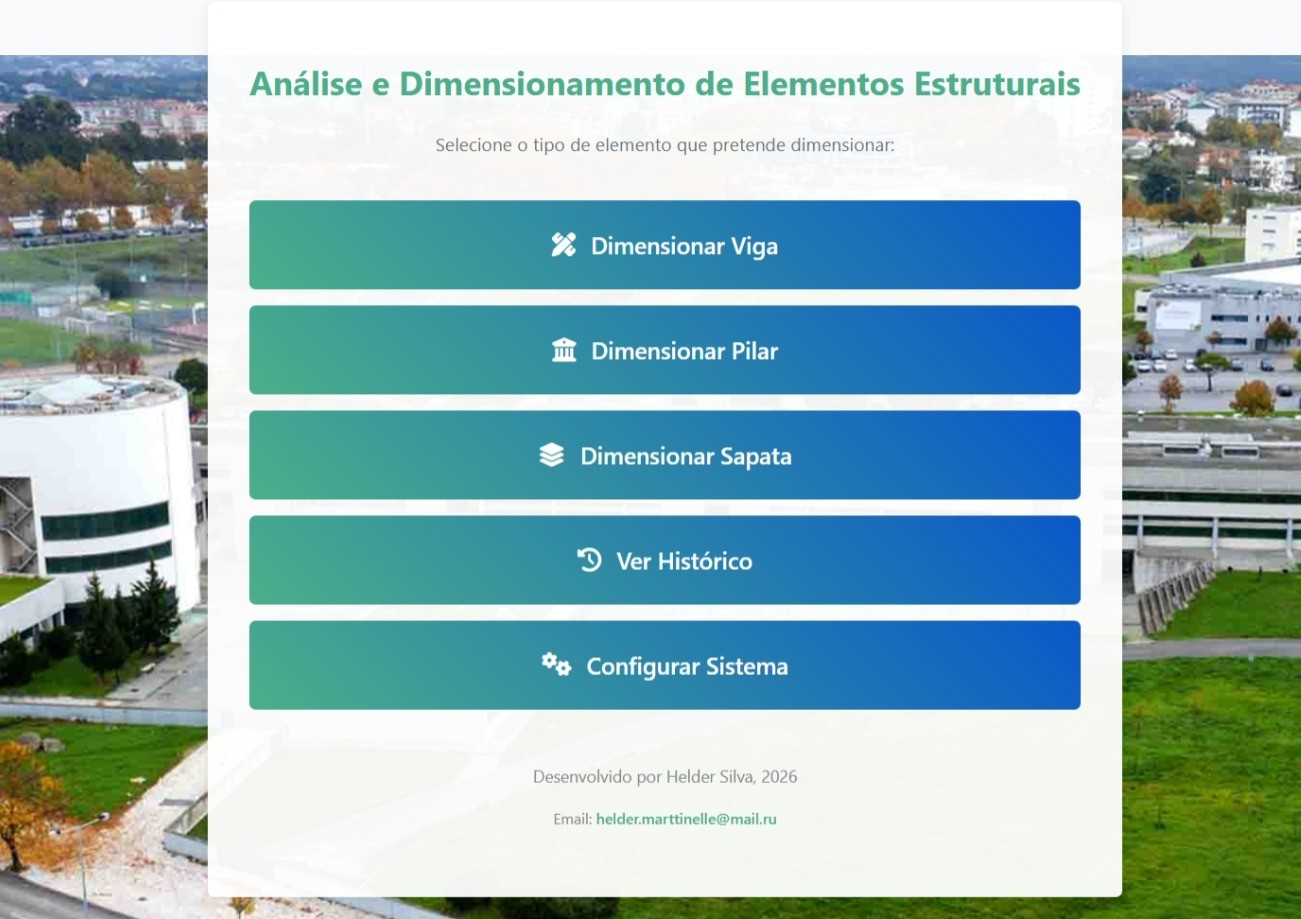
\includegraphics[width=0.9\textwidth]{Figuras/Menu_Inicial.jpg}
    \caption{Menu principal da aplicação com acesso aos módulos de dimensionamento.}
    \label{fig:menu_principal}
\end{figure}

\newpage
\subsubsection{Módulo de Vigas}
\paragraph{Entrada de Dados}

O formulário solicita as características geométricas da secção ($b, h$), as propriedades dos materiais (classes de betão e aço) e o esforço de cálculo ($M_{Ed}$) ver Figura \ref{fig:viga_input}.

\begin{figure}[htbp]
    \centering
    {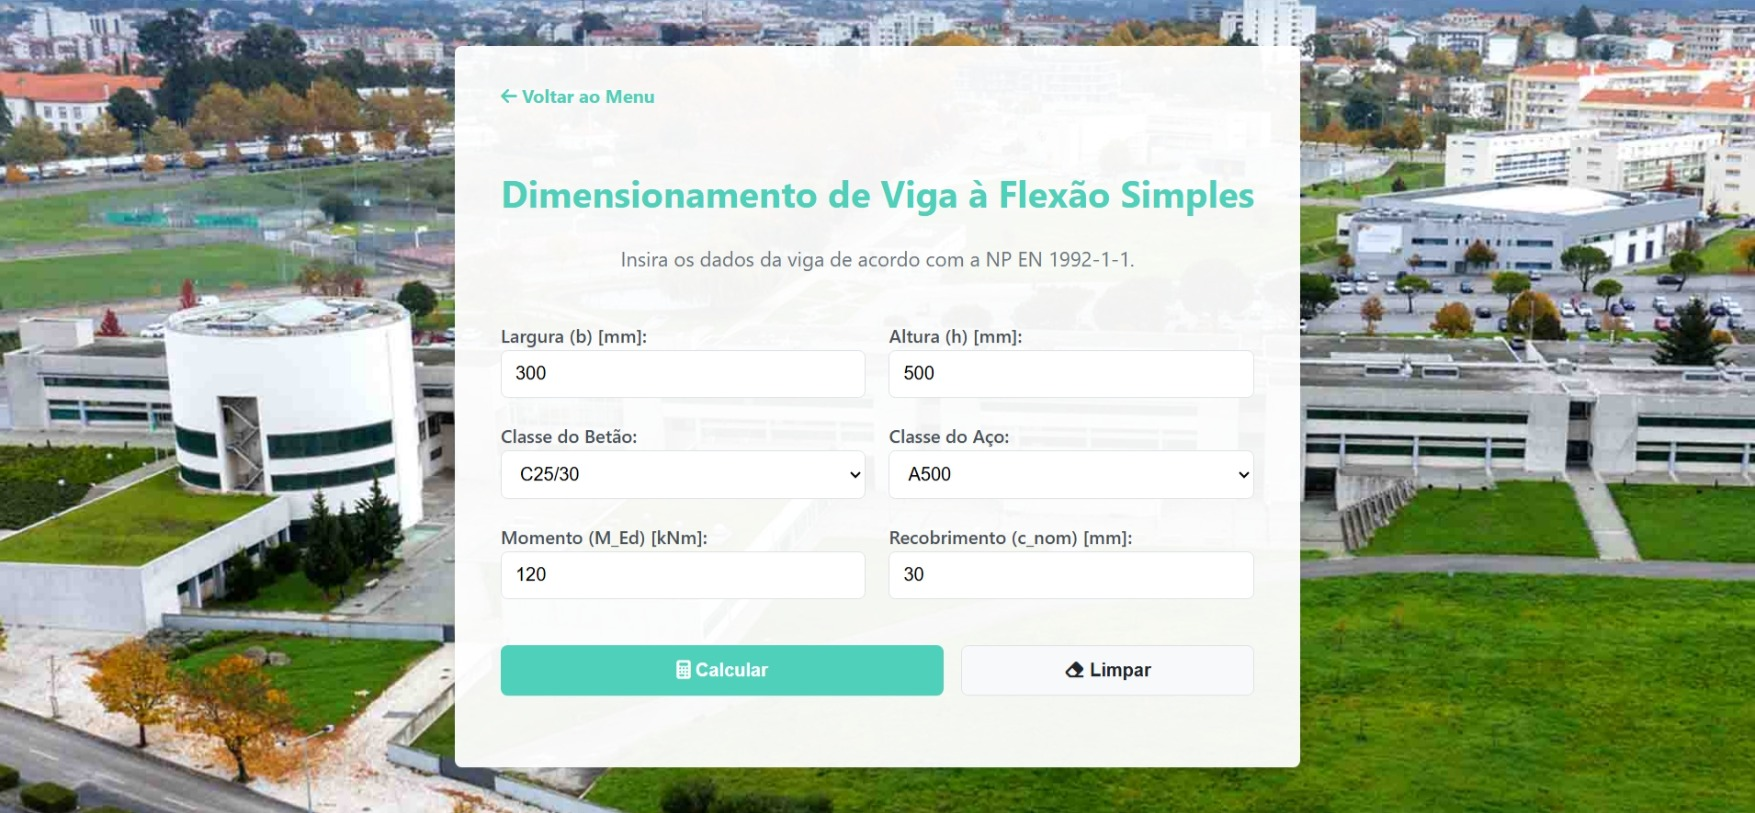
\includegraphics[width=0.89\textwidth]{Figuras/Viga.jpg}}
    \caption{Formulário de entrada de dados para o dimensionamento de elementos do tipo viga.}
    \label{fig:viga_input}
\end{figure}

\paragraph{Visualização de Resultados}
Após o cálculo iterativo, a aplicação apresenta a solução ótima de armadura e o desenho vetorial da secção. A visualização completa da interface com os resultados encontra-se no apêndice I.

\subsubsection{Módulo de Pilares}

\paragraph{Entrada de Dados}
Além da geometria e materiais, o utilizador define as condições de fronteira no topo e na base através de ícones gráficos, essenciais para o cálculo da esbeltez, ver Figura \ref{fig:pilar_input}.

\begin{figure}[htbp]
    \centering
    {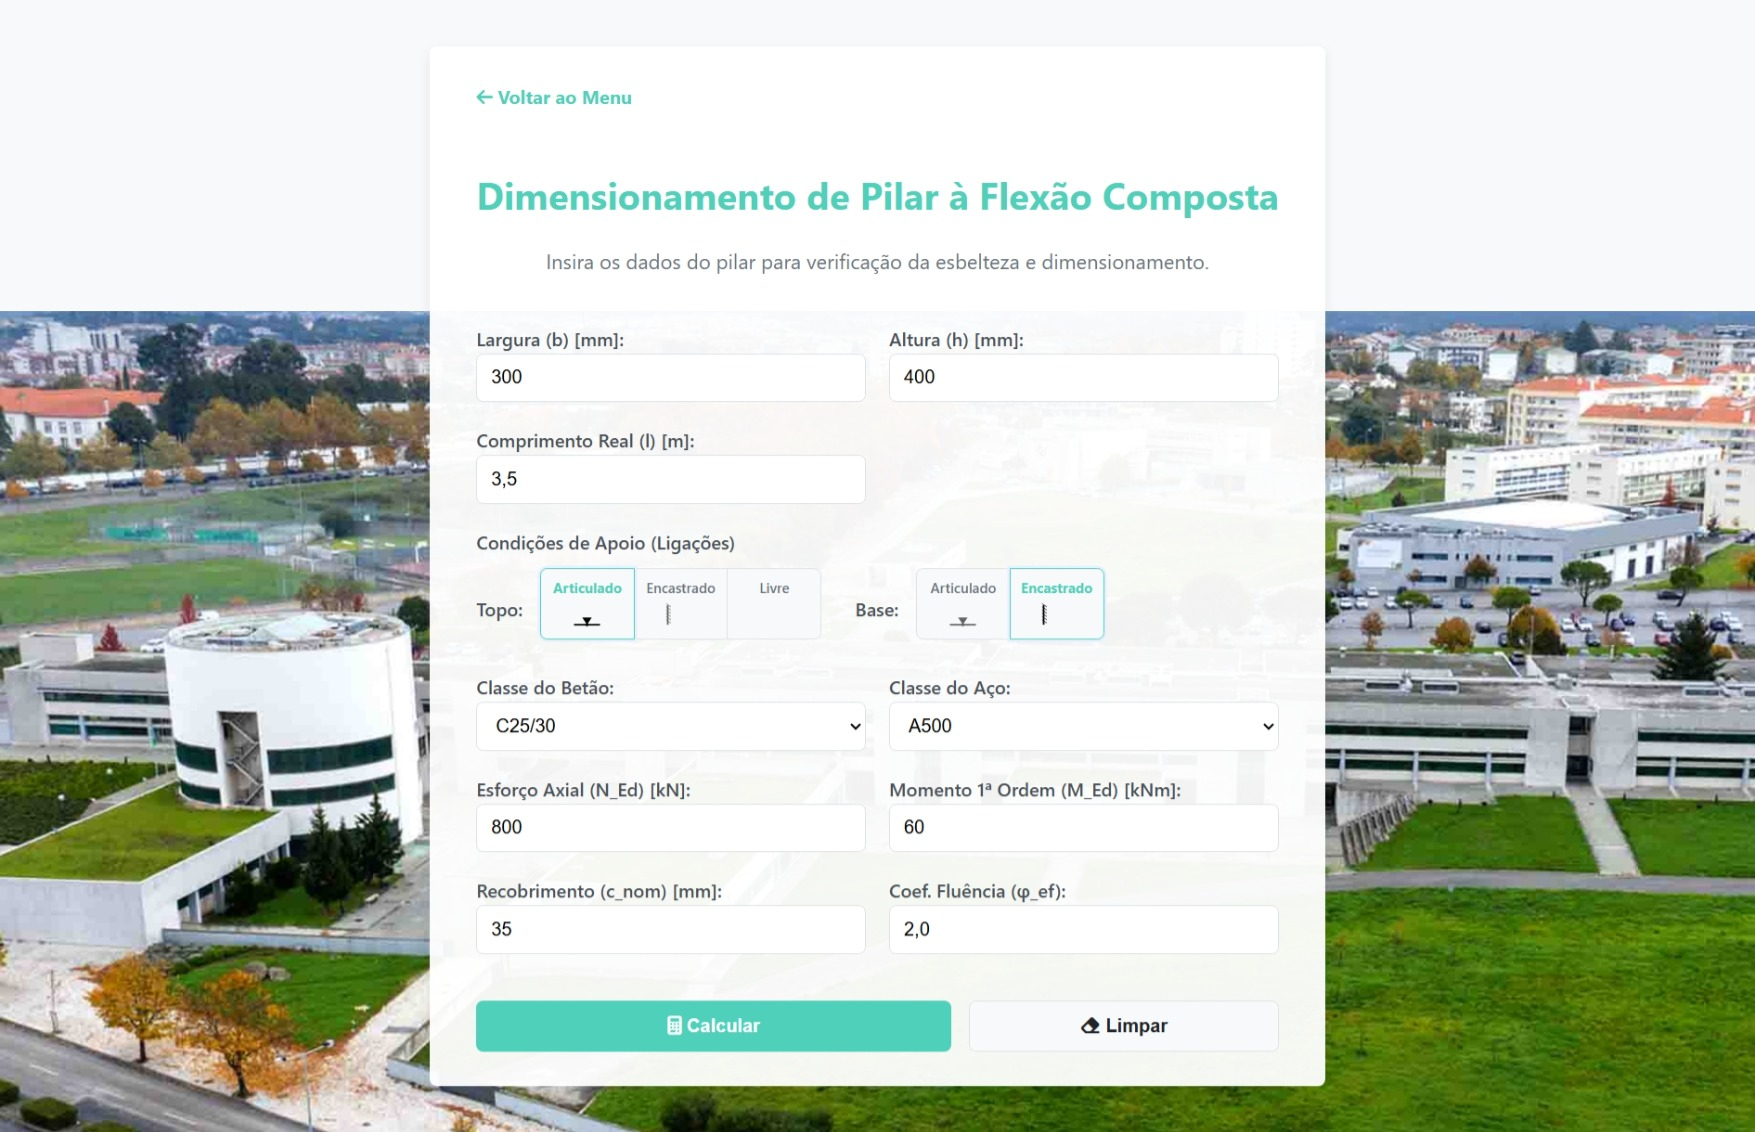
\includegraphics[width=0.88\textwidth]{Figuras/Pilar.jpg}}
    \caption{Formulário de entrada de dados para o dimensionamento de elementos do tipo pilar, com seleção visual das condições de apoio.}
    \label{fig:pilar_input}
\end{figure}

\paragraph{Visualização de Resultados}
O sistema apresenta a verificação de instabilidade e a armadura simétrica calculada. O desenho gerado ilustra a distribuição dos varões nas quatro faces. A interface de resultados pode ser consultada no no apêndice J.

\subsubsection{Módulo de Sapatas}

\paragraph{Entrada de Dados}
O utilizador introduz a tensão admissível do solo ($\sigma_{adm}$), as dimensões do pilar e os esforços atuantes ($N_{Ed}, M_{Ed}$).

\begin{figure}[htbp]
    \centering
    {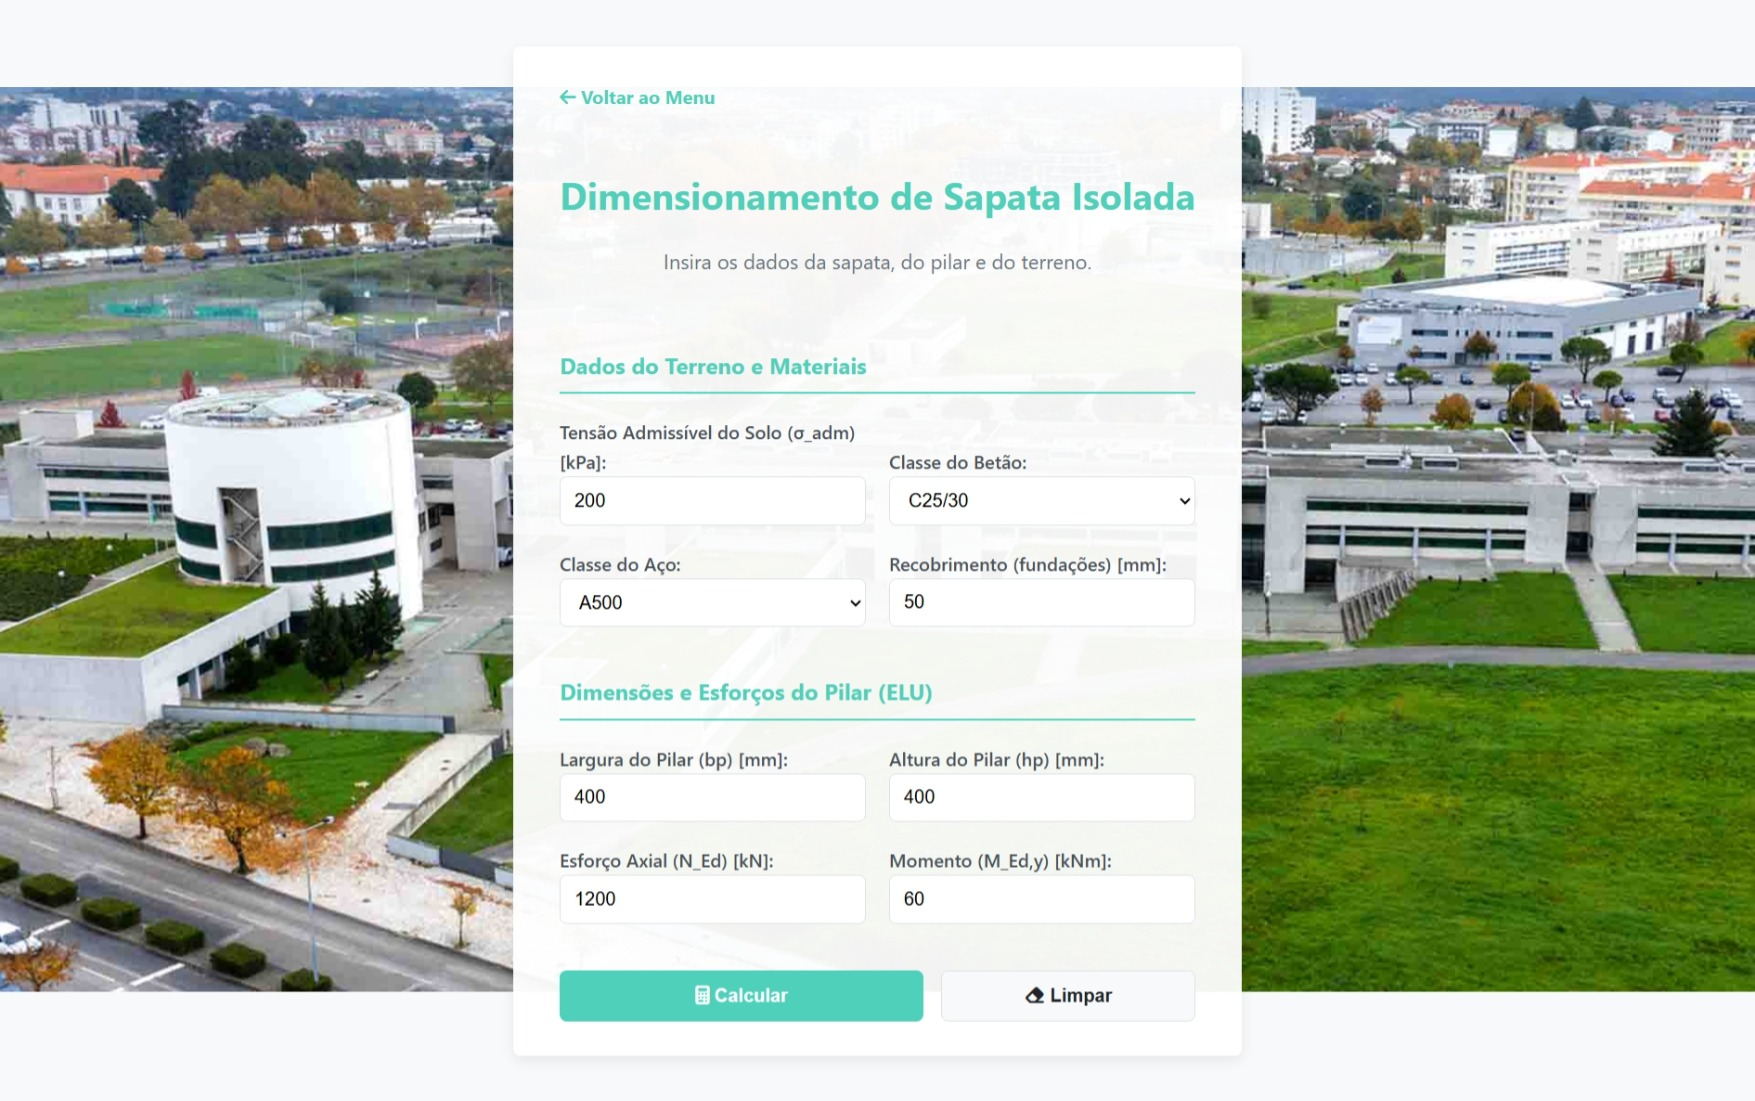
\includegraphics[width=0.9\textwidth]{Figuras/Sapata.jpg}}
    \caption{Formulário de entrada de dados para o dimensionamento de elementos do de sapata isolada.}
    \label{fig:sapata_input}
\end{figure}

\paragraph{Visualização de Resultados}


O resultado final inclui as dimensões em planta otimizadas e a altura verificada ao punçoamento, acompanhadas pelas vistas em planta e corte. A interface completa com estes resultados é apresentada no apêndice K.

\subsubsection{Ferramentas de Gestão}

\paragraph{Histórico de Cálculos}

Todos os dimensionamentos são guardados na base de dados. A tabela de histórico permite consultar e recuperar cálculos anteriores com interface completa
disponível no Apêndice G.

\paragraph{Configuração do Sistema}

O painel de configuração permite ao utilizador personalizar o aspeto visual da aplicação, alternando temas e cores, conforme ilustrado no Apêndice H.

\subsection{Disponibilização da aplicação}

A aplicação desenvolvida encontra-se disponibilizada em ambiente web na plataforma PythonAnywhere \cite{PythonAnywhere}, um serviço online de alojamento e execução de aplicações Python que permite publicar aplicações web na cloud. A versão funcional do sistema pode ser acedida online \cite{AppWeb_Tese}.
Paralelamente, o código-fonte da aplicação e dos algoritmos de dimensionamento encontra-se versionado no repositório GitHub \cite{RepoGitHub_Tese}. Esta separação entre ambiente de execução e repositório de código contribui para a organização do projeto, para a manutenção futura da aplicação e para a rastreabilidade das alterações efetuadas ao longo do desenvolvimento.


\subsection{Integração com análise matricial (Structrun)}

A aplicação está preparada para integração bidirecional com o Structrun \cite{Structrun} via JSON:

\begin{enumerate}
\item \textbf{Input}: gera \texttt{input.json} com geometria/nós/elementos.
\item \textbf{Processo}: invoca Structrun como subprocesso.
\item \textbf{Output}: lê \texttt{results.json} → alimenta automaticamente $N_\text{Ed}$, $M_\text{Ed}$.
\end{enumerate}

Esta cadeia completa (análise → dimensionamento) constitui perspetiva de evolução futura.